\chapter{Metode}\label{chap:metode}

\section{Litteraturstudie}
Denne mini-MTV's data og informationer er indhentet gennem litteraturstudier. Videnskabelig litteratur omhandlende videobaserede telesundhedsløsninger for hjemmepleje er søgt på følgende databaser: PubMed, Embase, CINAHL, Cochrane Library, Engineering Village og Google Scholar. Litteratursøgningsprocessen er udvidet til også at inkludere artikler identificeret ved kædesøgning i referencelister.

%\begin{figure}[H]
%\centering
%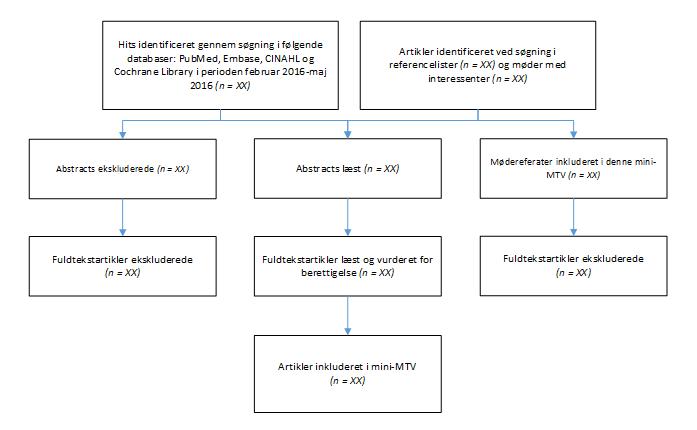
\includegraphics[width=1\textwidth]{Figurer/metode_flow.png}
%\caption{\label{fig:metodeflow}Flowdiagram over  litteraturstudie. Flowdiagrammet angiver litteratursøgningsprocessen og identificerer antallet af ekskluderede og inkluderede artikler i mini-MTV'en.}
%\end{figure}
%
%Emneord: \textit{Home Telemedicine, Telemedicine, Tele Care, Health Care, Tele Health Care, Caregivers, WebRTC, Cost, Cost effectiveness, Videoconference, Elderly, Nurses, Bandwidth, Home Care, Virtual Health Care, Telenursing, Virtual Visits, Workplace, Videocall, Driving, Municipality.}
%
%Ekskluderede artikler var telemedicinske problemstillinger vedrørende medicinsk behandling af patienter over distance. De inkluderede artikler omhandlede problemstillinger af telesundhedskarakter med fokus på virtuel hjemmepleje. Desuden artikler vedrørende brugen af WebRTC.  
%
%På baggrund af inklusions- og eksklusionskriterierne er antallet af artikler inkluderet i denne mini-MTV n = XX. Størstedelen af artikler er udenlandske, men er vurderet repræsentative for denne mini-MTV, idet parametrene, som undersøges er sammenlignelige. En fuldstændig generalisering er ikke mulig, idet sundhedsforholdene varierer i de forskellige lande, så en fuldstændig sammenligning på tværs af landegrænser er ikke mulig. 

\section{Generel dataindsamling}
Data er endvidere indhentet gennem møder med forskellige interessenter – Appinux, Netplan Care og medarbejdere i Favrskov Kommune. 

\subsection{Empirisk dataindsamling}
Med baggrund i de fokuserede spørgsmål har et stort fokus været at belyse borgernes og sygeplejerskernes oplevelser og erfaringer med virtuel hjemmepleje. Det har derfor været nærliggende at supplere litteraturstudiet og den generelle dataindsamling med en kvalitativ interviewundersøgelse for netop at opnå en indgående og detaljeret viden herom.\\
I forbindelse med evalueringen af \textit{Pilotprojekt Videokommunikation} blev der af Sundhedscenter Hadsten gennemført en lille kvalitativ evalueringsundersøgelse i form af strukturerede interviews med fire borgere og to sygeplejersker [Bilag 7, 1]. Data fra denne interviewundersøgelse er indhentet og kritisk vurderet med henblik på anvendelse som empirisk datagrundlag i denne mini-MTV fremfor at igangsætte en ny empirisk videns indsamling.

%\subsubsection{Diskussion af gyldigheden af den strukturerede interviewundersøgelse}
%Samlet set er den indhentede interviewundersøgelse fra \textit{Pilotprojekt Videokommunikation} vurderet gyldig, hvorfor det er valgt at medtage denne. Spørgsmålene svarede overens med denne mini-MTV's fokus. Dog efterlader denne ikke mulighed for generalisering. Formålet med at anvende kvalitativ metode har været at undersøge borgernes og sygeplejerskernes oplevelser med brugen af videoopkald som alternativ til fysisk hjemmeplejebesøg i forhold til Appinux' løsning i \textit{Pilotprojekt Videokommunikation} i Favrskov Kommune. Formålet har ikke været at lave et generaliserbart studie med resultater, som direkte kan overføres til andre lignende cases. Ved at sammenholde den empiriske dataindsamling med relevant videnskabelig litteratur samt viden indhentet ved møder med interessenter har det været muligt at opnå en dybere forståelse for borgernes og sygeplejerskernes perspektiv. 
%
%
%\section{Referencesystem}
%I denne mini-MTV anvendes Vancouver som referencesystem \cite{vancouver}. Bilag er vedlagt som en digital mappe og er organiseret med tydelig sporbarhed. Der henvises til bilag på følgende måde: [Bilag 1, 1.1].
%
%
  
	

